\documentclass[a4paper]{article}

\usepackage[spanish]{babel}
\usepackage[utf8x]{inputenc}
\usepackage{algorithm}
\usepackage[noend]{algpseudocode}
\usepackage{graphicx}
\usepackage{fontawesome}

\pagestyle{fancy} % Encabezado y pie de página
\fancyhf{}
% \fancyhead[L]{TP2 - Grupo 22 Data Wan Kenobi}
% \fancyhead[R]{Organización de Datos}
\renewcommand{\headrulewidth}{0.4pt}
% \fancyfoot[C]{\thepage}
\renewcommand{\footrulewidth}{0.4pt}

\begin{document}
\begin{titlepage} % Carátula
	\hfill
\includegraphics[width=6cm]{logofiuba.jpg}
    \centering
    \vfill
    \Huge \textbf{Trabajo Práctico 2}\\
    \textbf{Machine Learning}
    \vskip2cm
    \Large [75.06] Organización de Datos\\
    Segundo cuatrimestre de 2018 \\
    \bigskip
    \faGithub{}\quad \texttt{https://github.com/rozanecm/7506\_ml}\\
    \bigskip
    \bigskip
    Grupo: Data wan Kenobi
    \vfill
    \begin{tabular}{ || l | l ||} % Datos del alumno
      \hline
      
      ALUMNO & PADRÓN\\ [0.5ex]
      \hline \hline
      CACERES, Julieta & 96454\\
      \hline
      GARCÍA VILLAMOR, Delfina & 101154\\
      \hline
      FRUTOS RAMOS, Constanza M & 96728\\ 
      \hline
      ROZANEC, Matias & 97404\\
      \hline
  	\end{tabular}
    \vfill
    \vfill
\end{titlepage}

\tableofcontents % Índice general
\newpage

\section{Introducción}\label{sec:intro}

    El presente trabajo consiste en predecir si un usuario va a comprar o no un celular en la primer quincena del mes de junio.
    El resultado será expresado en la probabilidad de que dicho evento ocurra o no.\\
    Este problema puede ser analizado tanto como un problema de regresión, como un problema de clasificación binaria. Teniendo esto en cuenta se intenta usar ambas versiones de los algoritmos que se nombran a continuación.\\ 

\section{Tratamiento de datos}\label{sec:tratamiento}

    Al iniciar el trabajo se intentó resolverlo sin realizar tratamiento de los datos (a los datos categóricos se les aplicó la transformación One Hot Encoding para poder usarlos en las predicciones iniciales). Se usan en crudo, tal como aparecen en el csv a leer, y se agregan nuevas caracteristicas, como por ejemplo, a partir del timestamp obtener cual es la ultima visita.\\
    Se cree en un principio que mantener separados los registros de cada usuario ayuda a la predicción dado que ayuda a establecer relaciones temporales. Pero el máximo score alcanzado haciendo uso de los datos de esta manera es de 0.80. 
    Dado que las predicciones no eran sobre los usuarios sino sobre los registros (varios registros por usuario), luego debiamos obtener el promedio de dichas predicciones.\\
    De esta primera forma empezamos creando varias features diferentes, lo cual al hacer las predicciones de prueba siempre nos tiraba un score de 0.999 pero después cuando subíamos a Kaggle siempre obteníamos uno de 0.8 en el mejor de los casos. Esto nos dió una idea de que estabamos entrando en overfitting. Al analizar un poco más lo que teníamos se nos ocurrió que el problema podía estar en que la cantidad de features era demasiada comparada con la cantidad de registros con los que contabamos.\\
    
    Se decide cambiar la forma de tratar los datos generando una columna para cada usuario con varios features. Dichos features serán explicados a continuación.\\

\section{Features}\label{sec:features}

    \subsection{Selección de features}\label{subsec:seleccion features}

        Para la creación de features nos centramos en los eventos realizados por los usuarios y los timestamps de estos.
        Fuimos agregando más features a medida que avanzamos con el trabajo. Como dijimos anteriormente alcanzamos un punto donde tantos features nos generaban overfitting. Pero no solo eso, sino que también había features que subían más el score según con cuales otros los combinabamos. Así que no solo tuvimos que ir probando la cantidad de features adecuadas sino tambén cuales eran los mejores juntos.\\
        Para poder hacer esto último, utilizamos dos métodos:\\
        
        \begin{itemize}
            \item Uno es el "manual", donde ibamos probando con diferentes features un mismo algoritmo y guiándonos por lo que nos daba el score en los datos de test que separamos en un principio. Este método dió de hecho buenos resultados, pero requeria de nuestra atención y de probar las diferentes combinaciones nosotros. Esto no solo llevaba tiempo de trabajo de nuestra parte sino que además no es viable para probar varias combinaciones posibles. Como siempre se puede presentar el error humano, probando dos o más veces la misma combinación o salteandose combinaciones importantes porque no teníamos fe en que anduvieran. Para más o menos guiarnos en cuáles combinaciones queríamos probar de esta forma utilizamos RandomForest, el cual tiene la opción para mostrar las importancias de los features. Si bien a los resultados que nos daba los mirabamos con un poco de desconfianza, pero siempre decidimos que es mejor intentar todo lo posible.
            
            \item El otro método fue hacer uso del algoritmo SelectKBest, el cual es un algoritmo que ``corta'' la cantidad de features al k pasado seleccionando los mejores según una métrica de score pasada. Ahora, no solo teníamos el problema de que no sabíamos cuales eran las mejores columnas para el algoritmo de predicción utilizado sino que tampoco sabíamos la cantidad de columnas ideal para este. Para el segundo problema decidimos hacer uso de un GridSearch para el parámetro k de SelectKBest, de esta forma no solo buscábamos las mejores k columnas sino que también el k ideal. Pusimos para que nos busque con un k que iba de 1 a 37 (el total de features que teníamos en ese momento), para probar todas las posibles combinaciones. Al final tuvimos como resultado un k de 35 y el score en los test internos nos daba un 0.844. Decidimos subir las predicciones a Kaggle y estas nos dieron un score de 0.83... No mejoró lo que habíamos obtenido de la forma manual, pero se le acercó mucho, de lo que concluimos que era una buena forma de selección de columnas.
        \end{itemize}
        
    \subsection{Features creados}\label{subsec:features creados}

        \subsubsection{De los eventos}\label{subsubsec:eventos}
        Se hicieron varios features en base a la información de los eventos que teníamos:\\
        
        \begin{itemize}
            \item Cantidad de eventos totales: se contabiliza la cantidad de eventos total realizado por cada usuario.
            
            \item Cantidad por evento: luego se separa la cantidad para cada evento diferente.\\
            
            \item Support por evento: este feature lo sacamos del algoritmo apriori que hicimos para la exploración de datos, con el objetivo de ver la importancia de un conjunto de eventos. Lo que hicimos fue calcular el support de todas las n-tuplas posibles con todos los eventos, luego por cada usuario ver el conjunto de sus eventos. Le asignamos a cada usuario el support de la n-tupla de eventos correspondiente a los que hizo.\\
            
            \item Cantidad por evento dividido cantidad total: por cada evento, de los cuales ya contabamos con la cantidad de veces que un usuario lo realizó, se dividió esta cantidad por la cantidad total de eventos del usuario.
            
            \item Cantidad por evento dividido apariciones totales: siguiendo la misma idea que el anterior se dividió la cantidad por evento de cada usuario con la cantidad de apariciones totales de ese mismo evento (dentro de todos los datos con los que se contaba)
            
            \item Tambien se decide hacer uso de Mean Encoding sobre los eventos.
            
            \item Intentando explotar la importancia de este feature se decide multiplicar algunas columnas entre si de a pares.
        \end{itemize}
        
        \subsubsection{Del timestamp}\label{subsubsec:timestamp}
      
        Otra de las columnas de las que sacamos varios features es la del timestamp:\\
        
        \begin{itemize}
            \item Tiempo total: este es el cálculo del tiempo entre la primera aparición del usuario en el set de datos y la última aparición. Se lo puso en segundos.\\
            
            \item Tiempo promedio por día: se calculó el tiempo en horas de cada persona por cada día, y luego se realizó un promedio.\\
            
            \item Tiempo entre new y returning: recordemos que teníamos la columna new vs returning que nos indicaba si era la primera vez que ingresaba a la página o si estaba volviendo. Lo que hicimos fue calcular el tiempo entre el new de un usuario y el primer returning que hizo. Devuelta, esta diferencia de timestamps se la puso en segundos.\\
            
            \item Quincenas: como lo que querenos es predecir que dentro de una quincena un usuario va a comprar, lo que hicimos fue verificar si un usuario apareció en alguna quincena o no. En total se tienen 10 quincenas para el set de datos con el que contamos. Este mismo es un booleano.\\
            
            \item Dia: dado que en el análisis exploratorio realizado en el TP1 se vió que el mayor tráfico de usuarios se daba en los dias Martes, Miércoles y Jueves se decide agregar un feature que contabilice la cantidad de entradas de cada usuario en estos dias. Esto agregaba tres columnas, uno para cada dia.\\
            Luego, buscando disminuir las dimensiones, se usa el algoritmo a priori para obtener el support del dia de la semana, con un support mínimo de 0.4 se obtiene support para dichos dias, lo cual se condensa en una columna.
            
            \item Hora: Además del dia, se vió que hay horarios en los cuales hay más usuarios en el sitio. Nuevamente se hace uso del algoritmo a priori para obtener dicho support.
            
            \item Antes de agrupar los datos para trabajar con un registro por usuario se desplegó la información del timestamp obteniendo campos separados para el día (número), día de la semana (nombre), mes, hora y minuto. El día de la semana fue encodeado en un feature numérico. Todos estos features que resultaron ser numéricos fueron desplegados cada uno en una variable seno y otra coseno: de esta forma se mantuvo la naturaleza cíclica de los datos temporales. Una de las opciones al agrupar los datos por usuario fue tomar el promedio de cada caso.
        \end{itemize}
       
        \subsubsection{Cantidad de veces que vuelve al sitio}\label{subsubsec:Cant returnings}
        
        \begin{itemize}
            \item Se contabiliza la cantidad de veces que regresa al sitio, es decir cuando el valor de la columna ``new vs returning'' es de ``Returning''. \\
        \end{itemize}
        
        \subsubsection{De características varias de los usuarios}\label{subsubsec:caracteristicas usuarios}
        
        \begin{itemize}
            \item Channel más frecuente: para cada usuario le asignamos el channel por el que entró más veces. Como este es un string, luego se lo encodeó con target encoder.\\
            
             \item Device más frecuente: por cada usuario se calculó el device más usado por este (el de más apariciones). Como es un string se lo encodeó con target encoder.\\
             
             \item Modelo mas frecuente: por cada usuario se identificó el modelo mas buscado. El string fue codificado.
             
             \item Cantidad de modelos diferentes: Se calculó por usuario cuantos modelos distintos registraba.
             
             \item Condition mas frecuente: Se obtuvo por cada usuario la condición mas frecuente.
             
             \item Se agregó si ingresa al sitio en una fecha cercana al día de la madre (fecha de Brasil que es el pais con más usuarios), el cual es el 12 de marzo. Este feature no mejora la predicción.
             
             \item En el análisis exploratorio se vió que el mayor tráfico en el sitio se dió los dias Martes, Miércoles y Jueves, se agregan estos features contabilizando la cantidad de entradas en estos dias. Con este freature el score interno aumenta, pero no el de Kaggle, por lo cual se cree que puede ser causa de overfitting.
             
             \item Varios features categóricos que admiten una cantidad limitada de valores fueron desplegados en varias columnas, una por cada valor posible, colocando en cada campo la frecuencia por cada usuario para dicho valor, normalizado entre 0 y 1. De esta forma, cada usuario tiene una especie de puntaje para estos features.
             
             \item Varios features categóricos que admiten una cantidad mayor de valores fueron procesados mediante un imputer para rellenar los campos vacíos con estrategia \texttt{most\_frequent} y aplicando The Hashing trick. 
             
             
             \item Se hace uso de Mean encoding para algunas columnas con pocos datos tales como Storage, Channel y eventos.
             
        \end{itemize}
        
        \subsection{De versión de sistema operativo y de browser}
        \begin{itemize}
            \item En estos dos casos los valores originales contenían muchísimos valores distintos debido a la gran cantidad de versiones presentes de varios sistemas operativos/browsers distintos. Se decidió truncar los valores a la primera palabra, obteniendo de esta forma valores mucho más representativos, ya que puede decir algo del usuario si usa un browser u otro, pero no si, por ejemplo, usa chrome 54 o 63; la versión al final de cuentas agrega mucho ruido.
        \end{itemize}

        \subsubsection{De los supports}\label{subsubsec:supports}
        
        Se hace uso del algoritmo a priori para calcular la frecuencia de cada una de las columnas del dataframe de eventos. Se ajusta el suport mínimo según sea necesario para filtrar la información menos frecuente.
    
\section{Algunos detalles de implementación}
Para trabajar más fácilmente en la etapa de procesamiento de datos se decidió trabajar con herramientas específicas que trae la librería \texttt{sklearn}: se hizo uso de \texttt{Pipelines}, \texttt{ColumnTransformers} y \texttt{FeatureUnions}. Esto permitió tener todas las cosas referentes a las transformaciones de los datos juntas a mano, de forma que a la hora de querer realizar cambios en el procesamiento para probar varias cosas no hizo falta andar buscando las cosas a lo largo de un documento largo donde todo tiende a desorganizarse irremediablemente. La selección de transformaciones, columnas a las cuales aplicarlas y los hiperparámetros a ajustar se termina simplificando muchísimo de esta forma: definitivamente valió la pena invertir tiempo aprendiendo a usar estas herramientas.

\section{Algoritmos utilizados}\label{sec:algoritmos}
    
    Usamos varios algoritmos diferentes en busca de cuales eran los que mejor funcionaban con los datos que teníamos y con lo que buscabamos predecir.\\
    Antes de comenzar con probar lo algoritmos tenemos que definir qué tipo de problema tenemos. Dado que es un problema para calcular la probabilidad de que un usuario compre o no dentro de una quincena se lo puede tomar tanto como un problema de regresión como uno de clasificación.\\
    Una de las observaciones que hicimos al probar tanto los modelos de clasificación como de regresión de los distintos algoritmos, siempre sobre los mismos features y el mismo tratamiento de datos para poder hacer una comparación, es que muchas veces nos dan un poco mejor los modelos de regresión.\\
    
    \subsection{LightGBM}\label{subsec:lightgbm}
    
        LightGBM es un algoritmo de gradient boosting, utilizando árboles. A diferencia de otros algoritmos basados en árboles este contruye el árbol hoja por hoja mientras que el resto lo hace por niveles. Esto puede permitir reducir más el error. Pero se puede peligrar en entrar en overfitting, para evitar esto se tiene que tener cuidado con los hiper parámetros con los que uno crea el modelo. Principalmente el número de hojas y la profundidad máxima. A mayor prfundidad más exactitud y más peligro de caer en overfitting.
        Otro de las características que hacen más popular a este algoritmo es su rapidez y que no requiere de mucha memoria.
        
        Probamos con LGBM, tanto en Classifier como en Regressor. Siempre se vieron mejores resultados utilizando Regressor. Por esto los siguientes pruebas que hicimos fueron sobre el Regressor.
        Al principio se hizo una prueba simple con algunos features que teníamos al momento, y se conseguía un score interno del 0.7 en el regressor mientras que en el classifier uno de 0.?? Agregando un par de features más el score fue subiendo hasta que en un momento al seguir agregando bajó un poco. A esta altura decidimos entonces hacer uso del SelectKBest, usando GridSearch para encontrar el k que mejor se ajuste, para seleccionar las mejores columnas que se adaptaban a este algoritmo. De esta forma conseguimos un score interno de 0.843??, pese a que el interno no superaba lo que nos daba el mejor que teníamos en el momento decidimos subirlo para poder comparar, y el score final nos dió 0.83?? Por esta cercanía con el mejor score que conseguimos decidimos seguir trabajando sobre este algoritmo para ver si podíamos mejorar...\\
    
    \subsection{SVM}\label{subsec:svm}
    
        
    
        Se hizo un primer intento con SVM, tanto Classifier como Regressor, pero este nos daba un score muy bajo, uno de 0.5 en promedio (aún menos para el Classifier). Empezamos a probar con diferentes parámetros del algoritmo pero el score no subió mucho más. Dado este bajo puntaje se decidió dejarlo de lado.
        
    \subsection{KNN}\label{subsec:knn}
    
        Se utilizó K-Nearest-Neighbors, un muy sencillo algoritmo que se basa en para cada punto a clasificar buscar los k vecinos más cercanos, siendo k un hiperparámetro. Al encontrar estos vecinos es posible predecir la probabilidad para clasificar una clase.\\
        A la hora de usar este algoritmo siempre se tuvo en cuenta el orden de este mismo, ya que es de orden cuadrático. Por lo tanto es muy importante hacer un buen uso de los datos, para no utilizar un set de datos demasiado grande para KNN.\\
        Usando este se obtuvo un score de 0.5.. internamente y de 0.49 en Kaggle, estos para la forma de regresión del algoritmo. Como ha pasado con otros algoritmos y hemos dicho anteriormente, la versión de clasificación del algoritmo nos dió un puntaje un poco más bajo.\\
        Dado lo bajo del score que obtuvimos con este algoritmo y comparando con la precisión que obteníamos de otros algoritmos como XGB o LightGBM decidimos dejar de lado KNN. Aún así cuando se agregaron un par de nuevas features que lograron aumentar los puntajes de otros se decidió probar nuevamente el algoritmo, obteniendo resultados igual de bajos.\\
        Como ya se dijo anteriormente este es un algoritmo bastante sencillo y su simpleza también hace que no sea el mejor a la hora de las predicciones. Por lo que desde un principio tampoco se esperaba poder lograr muy buenos resultados con este mismo o mejorar lo obtenido.\\

    \subsection{LogisticRegression}\label{subsec:LogisticRegression}
    
        Haciendo uso de LogisticRegression se obtiene un score interno de 0.4285, por lo cual se decide no continuar probando este algoritmo.\\
        Realizando un Grid search se incrementa el score a 0.4313.\\

     \subsection{ExtraTreesClassifier}
        Utilizando diferentes combinaciones de feaures se procedió a probar este algoritmo, junto con la selección de parámetros mediante GridSearchCv se obtuvieron localmente valores de 0.9.. y en kaggle de 0.7..
        Los parámetros a buscar mediante grid search fueron n\_estimators, max\_features y min\_samples\_split.
        
    \subsection{ExtraTreesRegressor} 
    Luego de ultilizar ExtraTreesClassifier se decidió probar una regresión los resultados fueron similares.
    
    \subsection{Perceptron}
    Los resultados obtenidos en este caso no fueron comparables con los mejores scores hasta el momento. Con un score de 0.56 y sin lograr una mejora a través de GridSearch se decide no realizar un submit de las predicciones obtenidas con este modelo. Además la librería proporcionada por sklearn no provee una predicción probabilística para este algortimo.
    
    \subsection{Random Forest}\label{subsec:Random Forest}
    
       Se hace uso de Random Forest Regressor en varias oportunidades. Este algoritmo no supera en ninguno de los casos probados el score obtenido con XGBoost, por lo cual se decide usarlo simplemente para analizar la importancia de los features.\\
       Se hicieron ensambles en algunas oportunidades con XGBoost dado que los scores internos daban muy parecidos.
        
    \subsection{XGBoost}\label{subset:xgboost}
        
        Usando los features de Cantidad Total de eventos, Cantidad de cada evento por separado, algunas multiplicaciones con la columna 'ad campaign hit' y la separacion en quincenas se obtiene un score de 0.839. Luego se hace uso de RandomizedSearch con StratifiedKFold y se incrementa el score a 0.844. \\
        Calculando la importancia de estos parámetros con Random Forest se obtiene el siguiente resultado:\\
        \begin{figure}
              \centering
                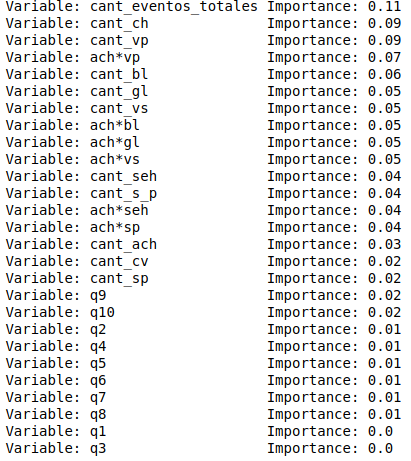
\includegraphics{Screenshot from 2018-11-29 23-14-50.png}
              \caption{Random Forest}
              \label{fig:ejemplo}
            \end{figure}
        Se remueven los features cuya importancia es menor a 0.04 para random Forest, se recalcula el score y se ve una baja del mismo a 0.7964.\\
        Este resultado es el segundo mejor obtenido en Kaggle. El mejor resultado se obtiene haciendo uso de XGBoost Classifier.
    
   
    \subsection{Ensambles}\label{subset:ensambles}
            
        \subsubsection{Ensamble XGB y LGBM}\label{subsubset:ensamble xgb lgbm}
            
            Dado que con XGBoost y con LightGBM obtuvimos buenos resultados, se decidió hacer un ensamble entre estos. Para esto calculamos el mean entre los resultados que nos daban ambos algoritmos y tomar esto como resultado final. El score interno que logramos de esta manera nos daba de un 0.83.
            Cabe aclarar qué versión de estos dos algoritmos tomamos para hacer el ensamble.\\
            En un principio se utilizaron los parámetros que mejor nos habían dado resultados en cada caso por su cuenta, y se utilizó la metodología de GridSearch junto con SelectKBest para la selección de las features a utilizar. Con esto conseguimos un 0.82.\\
            Pero un poco en desconfianza de esta metodología nuevamente se tomo los dos modelos, pero esta vez se utilizaron todas las features disponibles. De esta forma conseguimos un score de 0.83.\\
            Dado que de esta última forma conseguimos mejores resultados se decidió seguir trabajando sobre esta, solo que ahora cambiando un par de los hiper parámetros utilizados en los modelos. Partimos desde los parámetros que nos habían dado buenos resultados en un principio y empezamos a modificar algunos, de a poco y de a uno por vez, para poder ver como afectaba al resultado. Para esto además se tomó en cuenta qué significaba cada parámetro. Por ejemplo, ciertos parámetros de ambos algoritmos que sirven más que nada para evitar el overfitting (dar ejemplos) se dejaron de lado, ya que en nuestro caso queríamos aumentar la precisión. Y nos pareció lo mejor enfocarnos en aumentar esto y después cuando vieramos que entramos en overfitting intentar ajustar los parámetros nuevamente para salir de este mismo. De esta forma terminamos consiguiendo un score de 0.84 interno.\\
            Tener en cuenta que nuestro mejor resultado en Kaggle se consiguió con un score de 0.86 interno, con XGB.\\
            
            
    \subsection{Conclusión}\label{subset:conclusion}
        Se concluye que el mejor algoritmo es XGBoost para realizar esta predicción dado que en todos los casos el score obtenido con dicho algoritmo es mejor al obtenido con cualquier otro algoritmo.\\
        Se detecta que los features relacionados con los eventos son los mas importantes. A su vez la separación entre quincenas agrega información útil para el algoritmo. Del resto de las columnasse deduce que no agregan información útil a los algoritmos dado que no incrementan el score. 

\end{document}